\documentclass[12pt,a4paper]{article}

\usepackage[utf8]{inputenc}
\usepackage[T2A]{fontenc}
\usepackage[ukrainian]{babel}
\usepackage{geometry}
\geometry{
    left=2cm,
    right=2cm,
    top=2cm,
    bottom=2cm
}

\usepackage[table]{xcolor}
\usepackage{amsmath}
\usepackage{graphicx}
\usepackage{subcaption}
\usepackage{multirow}
\usepackage{makecell}
\usepackage{pdflscape}
\usepackage{array}
\newcolumntype{C}[1]{>{\centering\arraybackslash}m{#1}}

\usepackage[
  unicode,
  pdftitle={ІО-41, Давидчук А.М., Теорія ймовірностей та математична статистика, МКР №1},
  pdfauthor={Давидчук Артем},
  pdfsubject={Теорія ймовірностей та математична статистика}
]{hyperref}

\begin{document}

    \begin{titlepage}

        \begin{center}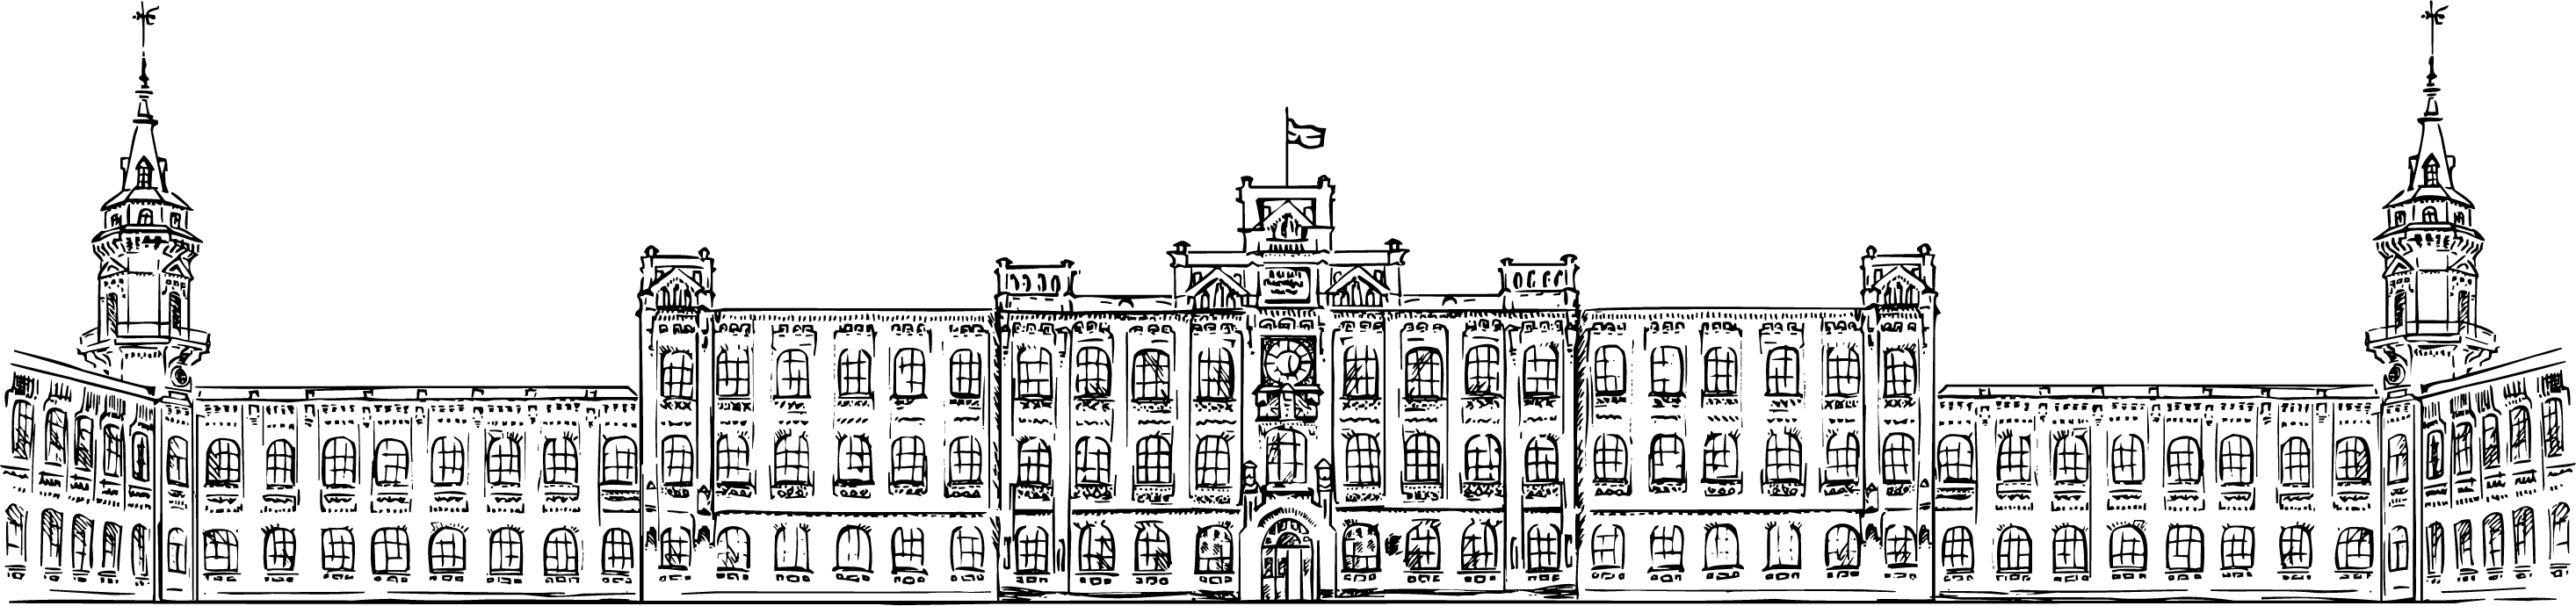
\includegraphics[width=0.7\textwidth]{../../TITLES/letterhead.png}\end{center}

        \begin{center}
            \large Національний технічний університет України\\
            «Київський політехнічний інститут імені Ігоря Сікорського»\\[1em]
            Факультет інформатики та обчислювальної техніки\\
            Кафедра обчислювальної техніки
        \end{center}

        \vfill

        \begin{center}
            \textbf{\LARGE Теорія ймовірностей та математична статистика}\\[2em]
            \textbf{\Large Модульна контрольна робота №1}\\[0.5em]
        \end{center}

        \vfill

        \begin{flushright}
            Виконав: студент 2 курсу ФІОТ, гр. ІО-41\\
            \textit{Давидчук А. М.}\\
            Залікова книжка № 4106\\[1em]
            Перевірив: \textit{Марковський О.\,П.}
        \end{flushright}

        \vfill

        \begin{center}Київ --- 2026\end{center}

    \end{titlepage}

    \begin{center} \textbf{\Large Вирішення} \end{center}

    \noindent
    Мій номер залікової книжки: 4106, звідси така задача:
    
    \begin{figure}[h]
        \centering
        
\includegraphics[width=\textwidth]{media/task.png}
    \end{figure}

    Побудуємо графічно рівномірний розподіл 3 чисел в інтервалі від 0 до 1:

    \begin{figure}[h]
        \centering
        
\includegraphics[width=0.8\textwidth]{media/t2.png}
    \end{figure}

    І значить нас цікавить випадок, коли хоча б одне число буде більше за 0.7, тобто складемо всі випадки, які нас задовільняють:

    \vspace{1em}

    001

    010

    011

    100

    101

    110

    111

    \vspace{1em}

    де, наприклад 001 -- означає, що числа $A$, $B \leq 0.7$, а число $C > 0.7$, а 110 -- $A, B > 0.7$ і $C \leq 0.7$, але рахувати 7 ймовірностей та потім їх додавати досить важко, і можемо скористатись властивістю доповнення:

    нехай подія $K$ -- це подія, при якій у нас хоча б одна з 7 комбінацій чисел спрацює, звідси  

    \[
    P(K) = 1 - P(\overline{K})
    \]

    де $\overline{K}$ -- це подія, що жодна із трьох чисел на більше за 0.7, і такий варіант один -- 000, ймовірність якої ми можемо порахувати, а звідси й $P(K)$.

    \newpage

    Так як у нас числа $A, B, C$ знаходяться в інтервалі $(0; 1)$, і площа кожного такого прямокутника = 1, то й висота = 1, тобто

    \[
    f(x) = h = 1
    \]

    Тепер потрібно порахувати такі площі (ймовірність того, що числа менше дорівнюють 0.7):

    \begin{figure}[h]
        \centering
        
\includegraphics[width=0.8\textwidth]{media/t3.png}
    \end{figure}

    Тобто для кожного числа ця ймовірність дорівнюю $1 \cdot 0.7 = 0.7$. А значить ймовірність того, що всі три числа одночасно будуть менші з 0.7 дорівнює

    \[
    P(\overline{K}) = 0.7 \cdot 0.7 \cdot 0.7 = 0.343
    \]

    Звідси ймовірність того, що максимум із 3 чисел буде більший за 0.7 дорівнює:

    \[
    P(K) = 1 - 0.343 = 0.657
    \]

    \vspace{3em}

    \noindent
    \textbf{Відповідь:}

    \begin{center}
        \boxed{0.657}
    \end{center}

\end{document}